
\subsection[Compilation MPTC]{Compilation du noyau MPTCP (machine
  test)}
\label{subsec:etatavanc:mininet-mptcp}

Pour la r�alisation du projet, nous utilisons une machine virtuelle
ubuntu 13.04 (32 bits) o� mininet est install� et est pr�t pour
utilisation :
\url{https://bitbucket.org/mininet/mininet-vm-images/downloads}.

Nous avons compil� le noyau linux contenant MPTCP (v0.88) dans une VM
de mininet (v2.10). Les paquets debian pour l'installation du noyau
MTPCP sur une VM de mininet est disponible :
(\url{https://www.dropbox.com/sh/y4ykck8rg6908ps/7V3lsV6Ggg}).

Cependant, l'architecture des machines pouvant �tre diff�rente, la VM
n'est pas fonctionnelle sur certaines des machines des membres du
projet. Par cons�quent, il est pr�f�rable de compiler soit m�me MPTCP
dans chaque machine. Le fichier ``.config'' utilis� pour la
compilation est disponible sur le premier git. La seconde option est
d'utiliser ``apt-repository'' selon les indications disponibles �
cette adresse
\url{http://multipath-tcp.org/pmwiki.php/Users/AptRepository}.


\subsection{Topologie}
\label{subsec:CR:topologie}

\subsubsection{Topologie simple}
\label{sec:simpletopo}

La premi�re topologie est inspir�e du \emph{testbed} de l'article de
R. Khalili \cite{pareto2013}, voir \fig{fig:topoMPTCP:A}. Nous avons
ajout�, � cette topologie, des routeurs priv�s entre le client et le
serveur \emph{MPTCP} pour disposer d'un nombre de sous-flots sup�rieur � deux.\\

\begin{figure}[H]
  \begin{changemargin}{-2.0cm}{0.5cm}
    \centering
    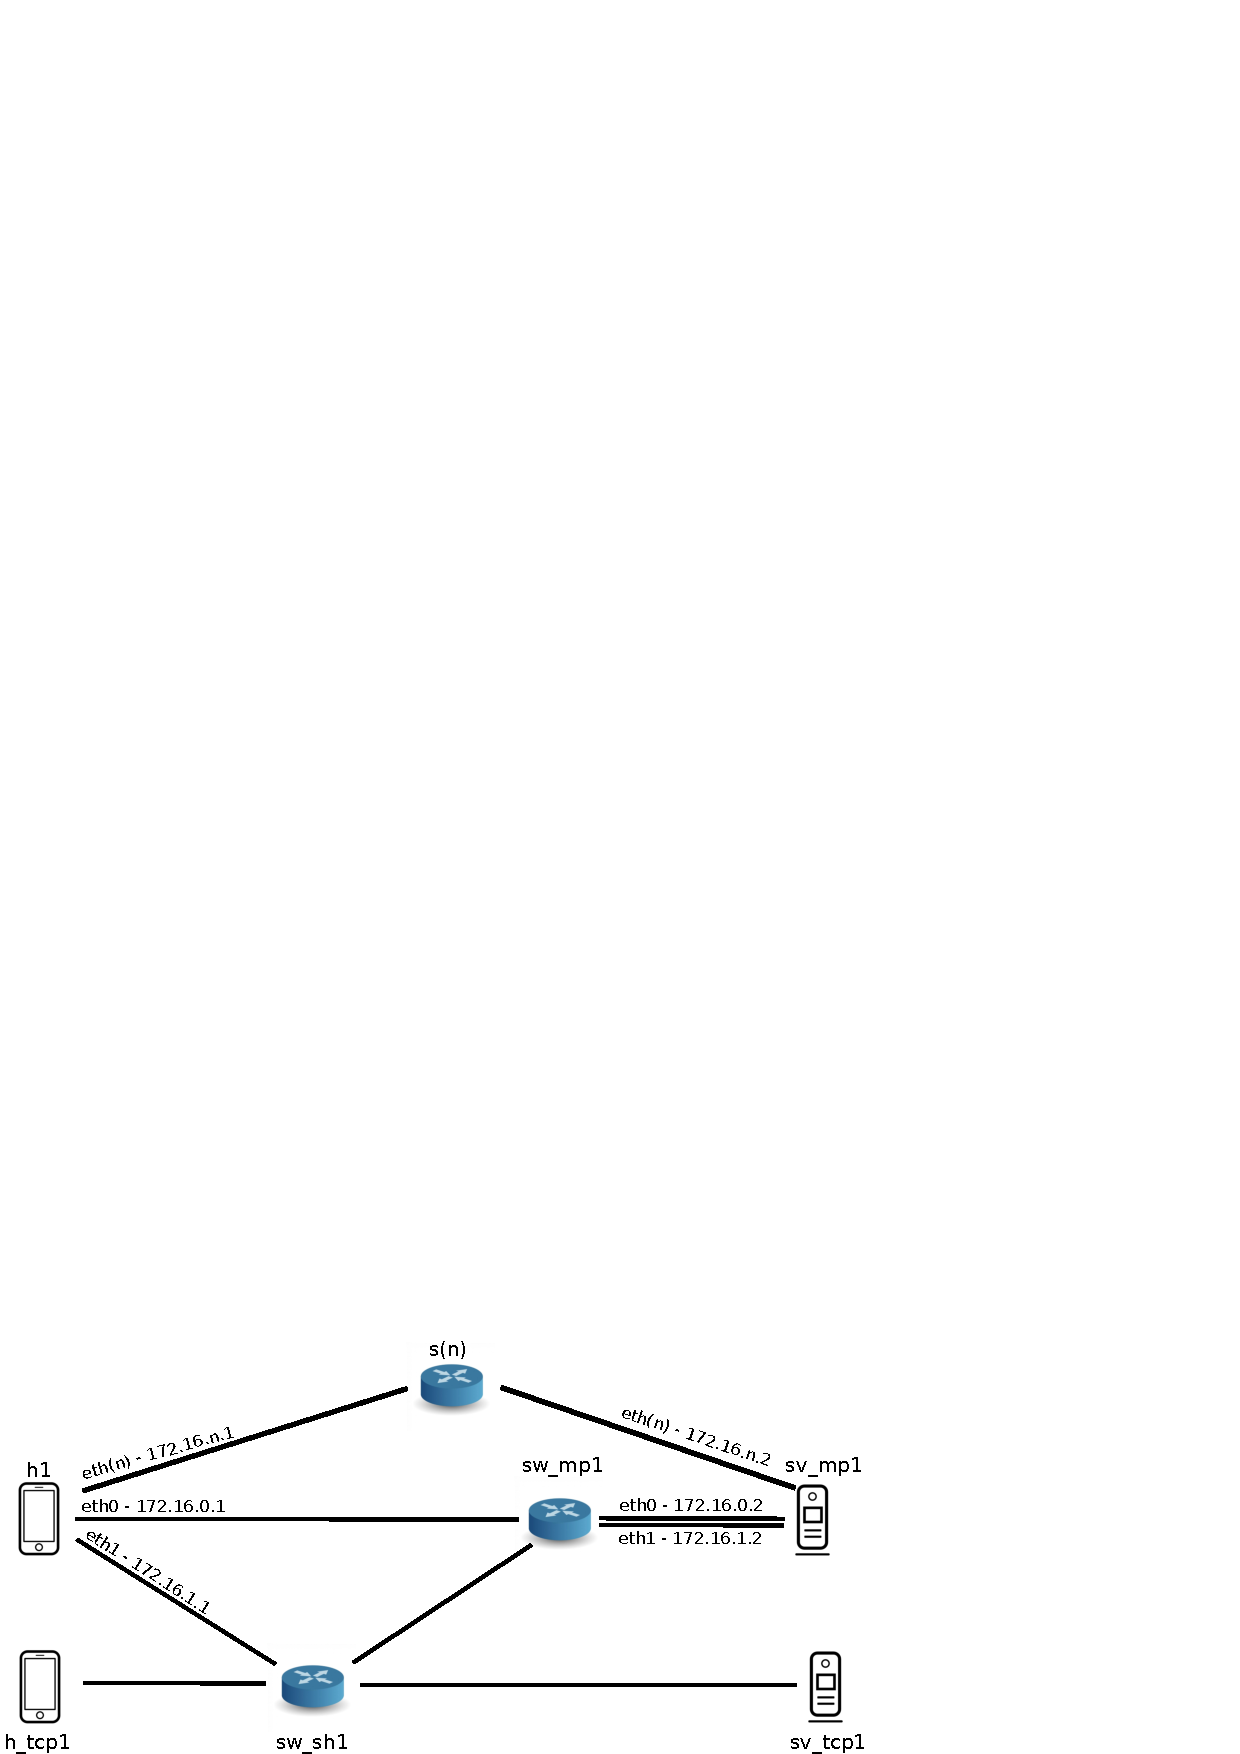
\includegraphics[width=0.7\textwidth]{../figures/mptcp_tcp/mptcp_tcp.pdf}
  \end{changemargin}
  \centering
  
  \caption{\textbf{Reproduction de la topologie de l'article de
      R. Khalili}. Le(s) \emph{switch(s)} ``S(n)'' ne sont pr�sent(s)
    que si le nombre de sous-flot est sup�rieure � deux. Pour n
    sous-flots, il y aura $n-2$ \emph{switchs} et $n-2$ liens
    suppl�mentaires. L'hyperviseur est connect� � tous les
    switchs. Pour se connecter via ssh aux h�tes, un \emph{switch} \og
    root \fg est cr�� et est connect� au \emph{switch} sw\_mp1 (non
    repr�sent� ici) voir utilisation CF linktobeadded.}
  \label{fig:topoMPTCP:A}
  
\end{figure}

\subsubsection{FatTree}
\label{sec:fattree}

Nous avions le choix entre plusieurs topologies pour r�aliser des
tests plus ��r�alistes��. Bcube, VL2, FatTree sont autant de
topologies utilis�es dans les \emph{data center} aujourd'hui. Pour des
raisons de facilit�s techniques, nous avons choisi d'impl�menter une
topologie FatTree.  Suite � notre recherche de documentation, nous
nous sommes retrouv�s confront�s � un choix�: plusieurs d�finitions du
FatTree sont ressorties, et certains d�tails constituaient de tr�s
nettes diff�rences au niveau de l'impl�mentation selon le mod�le
choisi.  La simplicit� d'impl�mentation de cette topologie repose sur
le fait qu'il s'agit d'un arbre dont la connectivit� entre les n\oe
uds augmente lorsqu'on se rapproche de sa racine.  Pour commencer,
nous nous sommes propos� de choisir l'approche la plus g�n�rale
possible en consid�rant un FatTree � 3 niveaux (Core, Edge, Hosts)�:



\begin{figure}[H]
    \centering
    \includegraphics[width=1\textwidth]{../figures/RAPPORT-FatTree1st.png}
    \caption{\textbf{Mod�lisation d'une topologie \emph{Fat-tree}}}
  \label{fig:topofattreeB}
  
\end{figure}


Cette mod�lisation consid�re que les switches sont tous identiques, et
poss�dent tous 36 ports.  Chacun des 2 switches du niveau racine
(\emph{Core switches}) dispose du m�me nombre de liens vers chacun des
4 switches du niveau interm�diaire, � savoir 9 liens vers chacun d'eux
(\emph{Edge switches}).  Ainsi, la moiti� des ports de chaque
\emph{Edge} switch, � savoir 18, sont d�di�s au niveau sup�rieur. Cela
laisse donc l'autre moiti� pour y connecter autant d'h�tes, � raison
d'un lien chacun. Le r�seau peut donc atteindre un maximum de 72
h�tes.  Cette repr�sentation a �t� choisie en raison de sa grande
flexibilit�. On peut ais�ment manipuler l'envergure du r�seau de test
(nombre d'h�tes, diversit� des chemins d'un h�te � un autre) en
fonction du nombre de \emph{Core switches} ou de \emph{Edge switches}
ainsi que du nombre de ports sur chaque switch.  Cependant, nous nous
sommes heurt�s � une difficult� technique lors de l'impl�mentation de
cette version du \emph{FatTree}. En effet, mininet ne supporte pas les
liens multiples entre switches, ce qui a r�sult� en une diversit� de
chemins entre h�tes insuffisante pour donner de l'int�r�t � une
simulation de MPTCP. Nous avons donc du revoir nos plans et nous
pencher sur un
nouveau mod�le de \emph{FatTree}.\\




Dans la nouvelle version de notre topologie, il n'y a plus lieu de
parler de multiples liens entre switches�; ils sont tous
interconnect�s par des liens uniques. Le probl�me de la diversit� des
chemins est r�solu par la transformation du \emph{FatTree} � 3 niveaux
en un \emph{FatTree} � 4 niveaux. Nous avons effectu� la s�paration du
niveau interm�diaire (\emph{Edge}) en 2 sous-niveaux. Les switches
connect�s au niveau 1 (\emph{Core}) seront appel�s \emph{Aggregation
  switches}, et ceux connect�s aux h�tes resteront les \emph{Edge
  switches}. La topologie ainsi obtenue est sch�matis�e ci-dessous.

\begin{figure}[H]
    \centering
    \includegraphics[width=1\textwidth]{../figures/RAPPORT-finalfattree.png}
  \caption{\textbf{Mod�lisation d'une topologie \emph{Fat-tree}}}
  \label{fig:topofattreeB2}
  
\end{figure}


Nous avons d�sormais 4 Core switches, 8 switches de niveau 2
(\emph{Aggregation}) et autant au niveau 3 (\emph{Edge}), ainsi que 2
h�tes pour chaque \emph{Edge switch} pour un total de 16
h�tes. L'interconnexion entre les sous-niveaux 2 et 3 est quelque peu
particuli�re�: sont regroup�s par clusters de 2 les \emph{Aggregation
  switches}, puis associ�s � un cluster de 2 \emph{Edge switches}. On
obtient ainsi 4 clusters de 4 switches r�partis sur les niveaux 2 et
3. Dans chacun de ces clusters, les 2 \emph{Edge switches} sont
connect�s aux 2 \emph{Aggregation switches} (il n'y a bien s�r pas
d'interconnexion entre switches de m�me niveau, il s'agit d'une
structure arborescente), r�sultant en une duplication du nombre de
chemins possibles. De plus, les \emph{Aggregation switches} sont
chacun connect�s � 2 des 4 \emph{Core switches}, dupliquant � nouveau
le nombre de chemins possibles. En r�sulte que chaque cluster peut
s'assimiler � un \emph{Edge switch} du mod�le pr�c�dant, offrant une
connectivit� directe vers les h�tes autant que vers chacun des
\emph{Core switches}.


\subsection{Performance de MPTCP sur mininet}
\label{sec:CR:perfMPTCP:base}

Apr�s la compilation du noyau, pour v�rifier le fonctionnement de
MPTCP nous avons mesur� le d�bit moyen en utilisant \emph{iperf} sur
la topologie A.

Les param�tres\footnote{param�tres par d�faut dans le noyau Linux}
utilis�s sont les suivants:


\vspace{1cm}
%\begin{tabular}{lp{\linewidth - 4cm}} 
\begin{tabular}{ll}
  \textbf{Param�tre}& \textbf{Valeur}\\
  \hline
  MSS& 1460 octets\footnote{Une erreur se produit lorsque nous fixons la valeur voir \pref{sec:annexe1:bugs:mininet}}\\
  window size& 85,3 Koctets\\
  d�lai par lien & 10 ms\\
  Algorithme de congestion& LIA \cite{rfc6356}\\
\end{tabular}
\vspace{0.5cm}


\subsubsection{Un exemple de d�monstration}
\label{sec:CR:perfMPTCP:unique}

Nous allons prendre, dans cet exemple, une connexion avec deux
sous-flots avec une capacit� individuelle de 100 Mbit/s. Voici la
commande pour g�n�rer cet exemple:
\begin{verbatim}
sudo python ./pyMPTCP -O exp001_TC --bw 100 -t 30 -n 2 --mptcp --bwm_ng
\end{verbatim}

Pour les d�tails de l'activation de MPTCP dans le noyau et
l'utilisation des arguments des scripts python, une notice est donn�e
en Annexe 1: voir sections \ref{sec:annexe1:usepyth} page
\pageref{sec:annexe1:usepyth} et \ref{sec:annexe1:mininetParserargs}
page \pageref{sec:annexe1:mininetParserargs}.

\vspace{0.5cm} Le RTT entre h1 et sv\_mp1 est de 44\,$\pm$\,11\,ms
(mesur� avec la commande \emph{ping}), ce qui correspond au RTT
attendu pour traverser deux liens aller-retour. La moyenne ici tient
compte du RTT du premier paquet qui est envoy� vers le contr�leur pour
que celui-ci �tablisse le chemin vers le serveur.

L'argument ``-\,-bwm\_ng'' permet de lancer Bandwidth Monitor
NG\footnote{\url{http://www.gropp.org/?id=projects&sub=bwm-ng} }
(bwm-ng). Cette application mesure plusieurs param�tres: le nombre
d'octets, de paquets, le d�bit entrant ou sortant passant par chacune
des interfaces de l'h�te sond�. La figure \ref{fig:MPTCP-perfbwm-ng}
repr�sente le d�bi entrant enregistr� au serveur pour ses deux
interfaces. Nous observons pour deux sous-flots aux capacit�s
identiques et au co�t identique, que le d�bit mesur� est quasi
similaire (une diff�rence de quelques paquets est observ�e).

\begin{figure}[htb]
    \centering
    \includegraphics[width=0.7\textwidth]{../figures/bw-single.pdf}
    \caption{\textbf{D�bit entrant c�t� serveur.} �chantillonage : 2\,Hz.}
  \label{fig:MPTCP-perfbwm-ng}
\end{figure}

Pour mesurer le d�bit total g�n�r�, nous effectuons une moyenne des
d�bits totaux mesur�s toutes les secondes par \emph{iperf} entre 5
secondes apr�s le d�but de la connexion, et 1 seconde avant la fin de
la connexion. Nous observons pour cet exemple, c�t� serveur, un d�bit
maximal de 168\,Mbit/s. Ce d�bit est coh�rent par rapport aux mesures
de d�bit \emph{via} bwm-ng.


\subsubsection{Variation du d�bit maximal par lien}
\label{sec:CR:perfMPTCP:nsousflots}

Pour conna�tre les limites de nos simulations, nous avons fait varier
la capacit� de chaque sous-flot, ainsi que le nombre de sous-flots
dans la topologie A.

\begin{figure}[htb]
    \centering
    \includegraphics[width=0.7\textwidth]{../figures/bw-coupled.pdf}
    \caption{\textbf{D�bit total mesur� en fonction de la capacit� du
        sous-flot.} Les d�bits sont mesur�s avec \emph{iperf} pour une
      connexion TCP classique et une connexion MPTCP contenant de 2 �
      6 sous-flots.}
  \label{fig:MPTCP-perf-subflow-bw}
\end{figure}

Le d�bit totale mesur� au serveur cro�t lin�airement avec
l'augmentation du nombre de sous-flots pour des capacit�s par lien de
10 � environ 100\,Mbit/s. Cette phase est en ad�quation avec le but de
MPTCP : augmentation des performances \cite{rfc6182}. Cependant, pour
les liens aux capacit�s sup�rieures � 100\,Mbit/s, les performances
d�croissent rapidement et tombent en dessous des performances d'une
simple connexion TCP ce qui viole la nature m�me de MPTCP .

Ce probl�me pourrait �tre expliqu� par une utilisation non optimale
de la capacit� des sous-flots. Le \emph{bandwidth delay product} (BDP)
implique une taille minimale du tampon de r�ception. Pour un d�bit de
1000\,Mo et un RTT de 44\,ms, la taille minimale du tampon est de
5,5\,Mo. Sachant que le tampon de r�ception\footnote{dans notre
  simulation la taille des tampons de r�ception est la m�me que la
  taille des tampons d'envoi.}  est partag� pour tous les sous-flots
d'une connexion MPTCP, la taille minimale du tampon doit suivre cette
formule \cite{rfc6824} :

\begin{equation}
  \label{eq:MPTCP:buffer}
  buffer\_size \geqslant max(\{RTT_i\}_{i \in [1,n]})*\sum_{i \in [1,n]} Bandwidth_{\{i\}}
\end{equation}

C'est � dire que la taille du tampon de r�ception doit �tre sup�rieure
ou �gal au produit du RTT le plus �lev� parmi tous les sous-flots et
la somme des capacit�s de tous les sous-flots. Cette taille de tampon
garantit l'utilisation optimale du lien lorsque des paquets
n�cessitent d'�tre retransmisent sur des sous-flots aux d�lais
lents. Dans notre simulation, il n'y a pas de perte de paquets, la
valeur minimale des tampons correspond au BDP le plus �lev�.

Pour les m�mes propri�t�s de liens, avec deux sous-flots, nous
obtenons une taille minimale de 11\,Mo. Mininet modife automatiquement
les tampons au lancement de la topologie et les valeurs utilis�es sont
les suivantes (en octets):

\begin{verbatim}
net.core.wmem_max = 16777216
net.core.wmem_default = 163840
net.core.rmem_max = 16777216
net.core.rmem_default = 163840
net.ipv4.tcp_wmem = 10240	87380	16777216
net.ipv4.tcp_rmem = 10240	87380	16777216
net.ipv4.tcp_mem = 19326	25768	38652
\end{verbatim}

Nous observons que le tampon maximal pouvant �tre allou� par socket
est de 16\,Mo environ ce qui est largement sup�rieur � la taille
requise. De plus en augmentant la taille du tampon, nous n'observons
pas d'augmentation de performances alors qu'en le diminuant, nous
observons une diminution du d�bit mesur� (voir
Fig. \ref{fig:mptcp:windowscale}).

\begin{figure}[!htb]
    \includegraphics[width=0.7\textwidth]{../figures/ws.pdf}
    \centering
    \caption{\textbf{D�bit mesur� en fonction de la taille de la
        fen�tre}. La taille maximmale de la fen�tre TCP est modifi�e
      avec l'argument '-w' avec \emph{iperf}. La taille obtenue est
      �trangement deux fois sup�rieure � la taille demand�. Le nombre
      de paquets indiqu� dans la l�gende correspond � la capacit� de
      traitement, en nombre de paquets, des routeurs.}
  \label{fig:mptcp:windowscale}
  
\end{figure}

Nous obtenons les m�mes r�sultats en modifiant la capacit� des
routeurs ou en modifiant les valeurs de la taille des tampons dans le
noyau (voir \ref{sec:annexe1:windowsize} page
\pageref{sec:annexe1:windowsize}) que ce soit les param�tres minimum,
par d�faut et maxium d'\emph{auto-tuning} de TCP (\emph{net.ipv4}) ou
les valeurs maximales ou par d�faut pour tous les type de connexions
(\emph{net.core}). Une v�rification de la charge CPU global avec
\emph{htop} ne montre pas une saturation des processeurs (environ
15\,\% d'utilisation) cependant, il reste � impl�menter \emph{cpuacct}
pour v�rifier la charge CPU par conteneur.


En effectuant des
recherches\footnote{\url{https://github.com/mininet/mininet/wiki/Introduction-to-Mininet\#what-are-mininets-limitations}}\footnote{\url{https://mailman.stanford.edu/pipermail/mininet-discuss/2014-January/003901.html}},
il semblerait que la limite du d�bit est li� aux n\oe uds Open vSwitch
sur Ubuntu 13.04, ce qui pour une dizaine de liens, limite la capacit�
maximale � environ 100 Mbit/s. De plus, il semblerait que l'activation
de \emph{auto-tuning} pour les tailles des tampons entra�nent une
basse significative des performances de MPTCP \cite{PKB13}. C'est pourquoi,
nous limiterons la capacit� des liens � de faibles valeurs.

\subsubsection{Variation du d�lai par lien}
\label{sec:compterendu:perf:d�lai}

Afin d'�valuer l'influence du d�lai sur le d�bit enregistr�, le d�lai
de tous les liens varie de mani�re sym�trique. Le co�t pour chaque
sous-flot reste donc identique.

Pour mesurer le d�lai de chaque sous-flot, nous avons utilis� la
commande \emph{ping}. Cette approche a �t� utilis�e car elle est la
plus facile � mettre en \oe uvre. Par manque d'espace disque (m�moire
SSD), l'utilisation de \emph{tcpdump} est r�serv�e pour les tests et
la recherche d'erreur. Cependant, il sera n�cessaire d'utiliser le
d�lai avec TCP car cette m�thode est plus fiable et l'utilisation
conjointe de \emph{ping} et d'\emph{iperf} produit une erreur (voir
\pref{sec:annexe1:bugs:mininet}).\\


\begin{figure}[tb]
    \centering
    \includegraphics[width=0.7\textwidth]{../figures/rtt.pdf}
  \centering
  
  \caption{\textbf{D�bit maximal mesur� en fonction du d�lai}. Le
    d�lai est du m�me ordre de grandeur pour tous les liens. Le RTT
    est mesur� avec la commande \emph{ping} avant le test avec
    \emph{iperf} qui dure 60\,s. Deux sous-flots sont utilis�s.}
  \label{fig:mptcp:rttisotrop}
  
\end{figure}

Nous observons que la modification du d�lai n'entra�ne pas de
diminution des performances pour les liens � faibles capacit�s
\fig{fig:mptcp:rttisotrop}. Ce qui est attendu vu que la taille des
\emph{buffers} et la capacit� des routeurs sont largement suffisantes
pour satisfaire � une augmentation de d�bit. Il reste alors � tester
ces cas dans des
conditions plus stringentes.\\

Pour les liens � haute capacit�, l'augmentation de d�lai entra�ne une
diminution du d�bit total. Pour 200\,Mbit/s et 400\,ms de RTT, il est
n�cessaire d'avoir environ 10\,Mo de tampon par sous-flot. Cependant,
il est possible que cette diminution drastique pour le lien �
200\,Mbit/s est en partie li�e aux probl�mes de simulation des d�bits
�l�v�s
avec mininet.\\


Nous constatons que la taille du tampon s'av�re �tre un param�tre
primordial dans les performances de MPTCP. Dans une utilisation
mobile, les deux sous-flots ont g�n�ralement des d�lais diff�rents
(par exemple, si on se base sur l'utilisation conjointe d'un acc�s
wifi, 3G ou/et ethernet). Dans la figure \ref{fig:mptcp:rttetTC}, nous
utilisons les m�mes param�tres que dans l'exp�rience pr�c�dente
cependant le premier sous-flot aura le m�me RTT (une dizaine de
millisecondes) pour toutes les exp�riences (exp�riences ``TC''). Nous
n'observons aucune diff�rence notable entre le cas o� les deux
sous-flots ont un RTT variable et dans le cas o� un seul des
sous-flots poss�de un RTT variable. L'exp�rience ``200 TC'' montre que
le d�bit est plus �lev� que l'exp�rience ``200'', cette diff�rence
peut �tre expliquer par une taille du tampon insuffisante.



\begin{figure}[htb]
    \includegraphics[width=0.7\textwidth]{../figures/prefixtc.pdf}
  \centering
  \caption{\textbf{D�bit total mesur� en fonction du d�lai d'un
      lien}. Le d�lai est modifi�e seulement pour le second lien dans
    la topologie A (exp�riences ``TC''). Le RTT est mesur� avec la
    commande \emph{ping} avant le test avec \emph{iperf} qui dure
    60\,s. Deux sous-flots sont utilis�s.}
  \label{fig:mptcp:rttetTC}
\end{figure}

\subsubsection{Choix du sous-flot en fonction du d�lai}
\label{sec:compterendu:perf:5choix}


Pour tester quels sont les sous-flots choisies par MPTCP dans une
connexion � \og faible \fg d�bit. Nous avons utilis� 5 sous-flots avec
diff�rents RTT. Le RTT de chaque sous-flot suit une sigmo�de (�quation
\ref{eq:sigmoide}).

\begin{equation}
  \label{eq:sigmoide}
  delay=min+\frac{max}{1+e^{\frac{x-x_{half}}{slope}}}
\end{equation}

Les param�tres\footnote{slope et $x_{half}$ ne sont pas utiles et
  permettent de contraindre le nombre d'exp�riences et la courbure des
  points d'inflexion.} utilis�s sont les suivants:

\vspace{1cm}
%\begin{tabular}{lp{\linewidth - 4cm}} 
\begin{tabular}{ll}
\textbf{Param�tre}& \textbf{Valeur}\\
\hline
delay& d�lai par lien\\
max& d�lai maximal par lien\\
min& d�lai minimal par lien\\
\end{tabular}
\vspace{0.5cm}

\begin{figure}[H]
    \includegraphics[width=0.7\textwidth]{../figures/TC5.pdf}
  \centering
  \caption{\textbf{D�bit re�u par interface c�t� serveur en fonction
      du RTT par sous-flot}. \emph{En haut}, RTT pour chaque
    sous-flot. \emph{Au milieu}, d�bit (Mbit/s) par interface. En bas,
    d�bit total (Mbit/s) enregistr� au serveur.}
  \label{fig:mptcp:sigmoid}
\end{figure}

Nous observons que le d�bit re�u est globalement �quivalent pour
chaque interface sauf pour l'interface ``eth4'' o� son d�bit est
inf�rieur � celles des autres pour des RTTs sup�rieur � 300\,ms. Le
d�bit total n'est que faiblement diminu�. En effet, la commande
\emph{iperf} envoie des paquets jusqu'� atteindre la capacit� de
chaque sous-flot. La l�g�re diminution des d�bits pour les d�lais long
est probablement
li�e au tampon de r�ception ou d'envoi.\\

Il est donc difficile de pr�dire les sous-flots utilis�s par
l'ordonnanceur. \emph{iperf} ne permet de contraindre le d�bit que
pour des paquets UDP. Nous avons donc int�gr�
\emph{iperf3\footnote{\url{https://github.com/esnet/iperf}}} � la VM
mininet
pour permettre de fixer le d�bit pour des paquets TCP.\\

L'utilisation d'\emph{iperf3} entra�ne une erreur qui n'a pas �t�
encore r�solue � la fin de la simulation (voir
\pref{sec:annexe1:bugs:mininet}) emp�chant toutes simulations
automatis�es. Nous avons donc choisi deux r�sultats caract�ristiques.

\begin{figure}[H]
    \includegraphics[width=0.7\textwidth]{../figures/bw-5_1_5_10_100_500.pdf}
  \centering
  \caption{\textbf{D�bit mesur� pour chaque interface}. Les RTTs pour
    les interfaces de eth0 � eth5 sont de 34, 38, 43, 137,
    552\,ms. Chaque lien a une capacit� de 10\,Mbit/s et le d�bit
    total g�n�r� par \emph{iperf3} a �t� fix� � 7,5\,Mbit/s.  }
  \label{fig:mptcp:bw151050}
\end{figure}

Dans la figure \ref{fig:mptcp:bw151050} et
\ref{fig:mptcp:bw1010500500500} nous observons que MPTCP envoie
pr�f�rentiellement les paquets dans les sous-flots � faible RTT. Il
�quilibre les charges dans les sous-flots o� le d�lai reste
raisonnable (sous-flot � RTT de 147\,ms dans la figure
\ref{fig:mptcp:bw151050}. Cependant pour les sous-flots � \og co�ts
\fg identiques, nous observons un effet de battement
(\emph{flappiness}). Il serait utile de mesurer le RTT au cours du
temps pour chaque sous-flot et d'�tablir si cet effet de battement est
li� � une variation du d�lai et ce pour l'algorithme LIA et OLIA
\cite{pareto2013}.

\begin{figure}[H]
    \includegraphics[width=0.7\textwidth]{../figures/bw-5_10_10_500_500_500.pdf}
  \centering
  \caption{\textbf{D�bit mesur� pour chaque interface}. Les RTTs pour
    les interfaces de eth0 � eth5 sont de 43, 43, 557, 557,
    557\,ms. Chaque lien a une capacit� de 10\,Mbit/s et le d�bit
    total g�n�r� par \emph{iperf3} a �t� fix� � 7,5\,Mbit/s.  }
  \label{fig:mptcp:bw1010500500500}
\end{figure}




\clearpage
%\subsection{Performance de MPTCP sur \emph{fat-tree}}
\label{sec:CR:perfMPTCP:fattree}


Nous avons effectu� divers tests de connectivit� en utilisant MPTCP
sur la topologie \emph{fat-tree}.


3- Routage Multipath

Apr�s documentation, nous avons d�couvert qu'il existait d�j� des
solutions � ce probl�me de routage. Mise � disposition du public sur
github, une impl�mentation d'un contr�leur con�u � l'intention des
r�seaux de Datacenter, et plus particuli�rement pour des topologies de
type FatTree, nous a permis de faire fonctionner MPTCP dans notre
r�seau, ainsi que d'effectuer nos tests de performance. Voici la
commande permettant de lancer ce contr�leur�:


\begin{verbatim}
~/pox/pox.py riplpox.riplpox --topo=ft,4 --routing=random --mode=reactive
\end{verbatim}


~/pox/pox.py�: fichier python d'ex�cution du contr�leur OpenFlow
riplpox.riplpox�: contr�leur Openflow destin� � la topologie FatTree d�crite plus haut (suppos� fonctionner �galement sur une topologie VL2)
--topo=ft,4�: s�lection de la topologie FatTree d�crite plus haut
--routing=random�: s�lection du type de routage (3 possibilit�s�: random, hashed, Spanning Tree)
--mode=reactive�: s�lection du mode d'ex�cution du contr�leur (3 possibilit�s�: reactive, proactive, hybrid)




Le fonctionnement de ce contr�leur openflow (appel� riplpox) est
relativement simple�: il se base sur une description statique du
r�seau afin d'�tablir la liste des chemins possibles entre chaque
h�tes. Par cons�quent, il faut s'assurer qu'il analyse exactement la
m�me topologie que celle virtualis�e par Mininet.  Il peut �tre lanc�
dans plusieurs modes diff�rents. Le mode proactive se contente de
r�f�rencer tous les chemins possibles � l'instant o� les switches sont
cr��s. Le mode reactive, plus int�ressant, actualise la liste des
chemins pour chaque nouveau flot. Dans le cadre de notre simulation,
la diff�rence est obsol�te puisque nous ne modifierons pas la
topologie pendant les tests. Cependant, l'un des objectifs de MPTCP
est d'assurer une meilleure r�action face � ce genre de probl�me�;
nous avons donc pr�f�r� utiliser le mode reactive qui, si nous avions
modifi� l'�tat des liens entre des phases de test successives, se
serait r�v�l� n�cessaire.











2/ Ex�cution des tests

Une fois finies la conception, la cr�ation et la configuration de
cette topologie plus complexe, nous nous sommes attel�s � int�grer
cette topologie dans notre environnement de tests. Suite aux
conclusions tir�es des simulations effectu�es sur la topologie A, nous
nous contenterons d'effectuer des tests avec une bande passante par
lien, pass�e en param�tre au script python lan�ant Mininet puis les
simulations (pyMPTCP.py), � 10 Mbit/s. De plus, notre topologie limite
l'usage de MPTCP � 4 sous-flots. Nous allons donc �tudier le d�bit
total de sortie en fonction du nombre de sous-flots actifs, et le
comparer au d�bit maximal th�orique et aux performances de TCP.

On s'attend � retrouver des r�sultats en corr�lation avec les tests
men�s sur la topologie A. En th�orie, l'�volution du d�bit total en
fonction du nombre de sous-flots devrait �tre lin�aire�; en effet, sa
valeur se r�sume � l'addition des d�bits des diff�rents
sous-flots. Cependant, suite aux r�sultats d�j� obtenus, on pourrait
penser que l'augmentation du nombre de sous-flots a des cons�quences
non d�sirables sur la rapidit� de transmission. �tant donn� le manque
de fiabilit� croissant de notre outil de simulation, Mininet, �
l'approche d'un d�bit de 100 Mbit/s et au-del�, et bien que nous nous
arr�tions � un d�bit maximal th�orique de 40\,Mbit/s, il est
envisageable que, m�me � ce stade, la progression de notre courbe s'en
retrouve affect�e.



\begin{figure}[!htb]
  \centering
  \includegraphics[width=0.6\textwidth]{../figures/RAPPORT-Perffattree.jpg}
  \caption{\textbf{Testbed MPTCP vs TCP\cite{pareto2013}}.}
  \label{fig:khalili}
\end{figure}

En utilisant, comme nous l'avons fait, des liens de 10\,Mbit/s, le
d�bit total est en th�orie limit� � 10*N, N �tant le nombre de
sous-flots utilis�s. De la m�me mani�re, une connexion TCP �tant
�quivalente � une connexion MPTCP � un seul sous-flot, celle-ci reste
constamment � 10\,Mbit/s. Nous avons choisi de repr�senter ces bornes
autour de notre courbe afin de mettre en valeur l'int�r�t de
l'utilisation de MPTCP par rapport au Single-Path TCP, tout en
essayant de constater les pertes induites par Mininet, dont nous
connaissons la teneur suite aux exp�rimentations pr�c�demment
effectu�es.  Suite � l'exploitation des chiffres obtenus par nos tests
sur cette topologie FatTree, nous constatons plusieurs faits qui
m�ritent d'�tre mentionn�s. Tout d'abord, Nous avons remarqu� que le
d�bit moyen de MPTCP avec 1 sous-flot est l�g�rement inf�rieur au
d�bit moyen du Single-Path TCP. Ceci peut s'expliquer par le fait que
MPTCP effectue de nombreux traitements suppl�mentaires, lesquels sont
totalement inutiles dans le cas de l'utilisation d'un unique
sous-flot. De plus, nous notons �galement qu'� partir d'un d�bit
d'environ 40Mbit/s, le d�bit exp�rimental de MPTCP commence �
s'�loigner significativement de la courbe du d�bit th�orique. Ceci
confirme que, outre le fait que la capacit� totale de chaque lien soit
moins bien exploit�e par MPTCP, notre simulateur atteint assez
rapidement ses limites.

Dans la pratique, MPTCP s'est r�v�l� capable d'atteindre un d�bit
total de plus de 50Gbit/s en utilisant des liens �
10Gbit/s. Malheureusement, les limitations de Mininet ne nous
permettront gu�re de d�passer les 100Mbits/s. Cependant, il est av�r�
que MPTCP permet effectivement d'exploiter une diversit� de chemins
afin de multiplier le d�bit total d'une connexion pair � pair.

\clearpage

Une partie de ce projet consistait dans un premier temps en l'�tude du
code de MPTCP et de la compr�hension de son fonctionnement, puis dans
l'impl�mentation d'un nouvel ordonnanceur de notre choix. Apr�s
discussions, nous avons d�cid� de placer deux personnes sur l'�tude du
code de MPTCP car il nous semblait important d'avoir une bonne
connaissance du fonctionnement du code et des principales structures
pour pouvoir impl�menter un nouvel algorithme d'ordonnancement.

\subsection{Etude de  l'algorihme de MPTCP}
 	\subsubsection{Explication de l'ordonnanceur}
 	Lors de l'�tude du code de MPTCP, nous avons �tudi� l'ordonnanceur d�j� impl�ment�. L'ordonnanceur de MPTCP tient dans la fonction get\_available\_subflow(), qui se trouve dans (\$SRC NOYAU)/net/mptcp/mptcp.output.c. Cela nous a �t� confirm� par Matthieu Coudron lorsqu'il a choisi l'ordonnanceur � impl�menter. Cette fonction retourne la socket sur laquelle sera envoy�e le prochain segment de donn�es et d�finit la taille du Maximum Segment Size (MSS). Nous allons vous expliquer comment marche cet algorithme. Mais pour cela il faut connaitre d'avance les structures principales que nous allons vous expliquer avant de commenter l'ordonnanceur.\\
 	Tout d'abord la structure mptcp\_cb signifie \emph{MPTCP control block} c'est la pierre angulaire de MPTCP. Elle est utilis�e dans pratiquement toutes les fonctions de MPTCP. Cette structure permet de superviser les diff�rents sous-flots utilis�s pour une connexion MPTCP. Elle permet aussi de d�cider s'il faut ouvrir ou fermer un sous-flot, elle r�ordonne les donn�es re�ues afin que l'application qui a besoin de ces donn�es les obtienne dans le bon ordre.\\
 	La structure sock (socket) et la structure sk\_buff (socket
        buffer) sont les m�mes que dans TCP. La socket permet de cr�er
        une liaison entre les machines : elle d�tient les informations
        n�cessaires � la transmission des donn�es; quant au socket
        buffer, elle permet de d�finir ce que doit envoyer une socket
        et permet de faire un tri sur les donn�es re�ues gr�ce au
        timestamps.  L'ordonnanceur impl�ment� dans MPTCP utilise,
        comme dans notre impl�mentation, le Smoothed Rount Trip Time
        (SRTT) pour d�terminer quelle socket enverra les donn�es. De
        ce fait, si le SRTT est petit, l'ordonnanceur utilisera plus
        souvent cette socket. C'est ce qui cr�e une faiblesse dans la
        s�curit� de la transmission alors qu'avec MPTCP, comme il y a
        plusieurs chemins, la complexit� peut �tre accrue s'il y a un
        �quilibrage dans l'envoie des donn�es entre les sous-flots.
        \bigbreak
        Nous allons maintenant nous int�resser � la fonction get\_available\_subflow() qui est l'ordonnanceur.\\
        L'algorithme se d�roule de la fonction suivante:
 	 \begin{itemize}
         \item Tout d'abord, il y a une v�rification sur le nombre de
           sous-flots ouverts dans la connexion MPTCP. Il est possible
           de r�cup�rer cette valeur gr�ce � la structure mptcp\_cb(
           $mpcb->cnt\_subflows$ ). On effectue ce test au pr�alable
           dans le cas o� il n'y aurait qu'un seul sous-flot, au quel
           cas, il suffit de renvoyer l'unique socket s'il est
           disponible. Pour tester la disponibilit� d'une socket, la
           fonction \emph{mptcp\_is\_available()} existe d�j�. Elle
           v�rifie qu'elle peut envoyer (v�rification des champs de la
           socket), que la connexion est totalement �tablie, que la
           socket soit �ligible et, que sa fen�tre d'envoi est
           suffisante. Si la fonction renvoie \emph{true} alors le
           sous-flot peut �tre �ligible pour envoyer des donn�es. On
           peut r�cup�rer les sockets via la structure
           $mpcb->connection\_list$ qui liste les sockets associ�es
           aux sous-flots.
         \item Sinon on regarde toutes les sockets associ�es � la connexion MPTCP et on distingue trois types de sockets: les backup sockets, lowpriority sockets et la meilleure socket.\\
           Dans cet algorithme, il y a des sockets qui ont une
           priorit� basse et qui ne serviront que s'il n'existe pas de
           sockets avec une priorit� plus grande que cette
           priorit�. C'est ce qu'on appelle les lowpriority
           sockets. Parmi toutes les sockets, on choisit celle qui a
           le plus petit SRTT. Et on la stocke dans la variable
           \emph{lowpriosk}. Bien qu'elle soit nomm�e lowpriority,
           elle a une fonction de backup mais c'est une socket
           �ligible contrairement � la backup socket.
\item Si il y a d'autres sockets qui non pas une faible priorit�, on compare le SRTT de ces sockets et on garde la socket avec le RTT le plus faible. Elle est stock�e dans la variable \emph{bestsk}.\\
Il y a aussi une backup socket qui sert au cas ou aucune des sockets d�crites ci-dessus ne peuvent envoyer un segment de donn�es : c'est le dernier recours car celle-ci est d�sign�e alors qu'elle ne permet pas la r�injection de donn�es. Elle sera stock�e dans la variable \emph{backupsk}. 
\item Maintenant que nous avons d�fini les diff�rents types de
  sockets, il faut savoir sur laquelle des trois sockets on va envoyer
  les donn�es; Si il n'y a que des sockets de backup, on envoie les
  donn�es sur la \emph{lowpriosk}. Sinon on envoie les donn�es sur
  la \emph{bestsk} si elle existe. Et s'il n'y a pas de
  \emph{bestsk}, on utilise \emph{backupsk}.
\end{itemize} 

 	\subsection{Choix de l'ordonnanceur}
        Pour le projet, il fallait choisir et impl�menter un nouvel
        ordonnanceur. Nous avions �mis plusieurs hypoth�ses pour ce
        nouvel algorithme. En accord avec les encadrants, il a �t�
        d�cid� de juste utiliser le SRTT des sockets pour faire notre
        impl�mentation.  \bigbreak
        Dans un premier temps, nous avons pens� impl�menter un algorithme assez simpliste mais qui permettait d'augmenter la s�curit� contre les attaques de type \emph{Man In The Middle}. C'est � dire que notre algorithme allait envoyer les segments de mani�re �quitable sur chaque sous-flots permettant l'envoi de donn�es. Cet algorithme avait pour vocation de rendre plus difficile la r�cup�ration d'informations en �coutant un sous-flot car avec l'algorithme actuel, si un attaquant voulait r�cup�rer un maximum d'informations, il lui suffisait d'�couter le sous-flot qui a le SRTT le plus faible. C'est ce que nous voulions �viter avec notre algorithme. Cependant apr�s de plus amples r�flexions, nous avons remarqu� que notre algorithme avait un grand nombre de d�fauts.\\
        En effet, MPTCP a �t� d�velopp� afin d'avoir une am�lioration
        des d�bits mais cet algorithme aurai emp�ch� cela si le d�bit
        d'un sous-flot �tait vraiment faible compar� aux autres
        sous-flots alors toute la connexion MPTCP ressentirait ce
        d�bit faible et cela influerai beaucoup sur les performances
        de MPTCP. C'est pourquoi cet algorithme n'a pas �t� choisi.
        \bigbreak Un compromis entre s�curit� et performances est
        n�cessaire pour que l'utilit� de MPTCP soit avantageuse par
        rapport � TCP. Il nous a �t� propos� de s�lectionner les
        \emph{k} meilleurs sous-flots d'un point de vue du SRTT et de
        faire un Round-Robin sur ces k sous-flots. \emph{k} �tant
        laiss� � notre appr�ciation. Cet algorithme est le meilleur
        compromis trouv� car il permet de ne pas envoyer de donn�es
        sur un sous-flot si son SRTT est trop grand, ce qui permet de
        garder une certaine rapidit� dans la transmission de donn�es
        et de garder une certaine s�curit� car le trafic passe de
        mani�re �quitable sur les \emph{k} meilleurs sous-flots.
\subsection{Impl�mentation de l'ordonnanceur}
Afin de pouvoir stocker les \emph{k} meilleurs sous-flots, on avait 2 choix.
\begin{itemize}
\item Soit un tableau.
\item Soit une liste chain�e.
\end{itemize}
Apr�s en avoir discut� entre nous, nous avons d�cid� d'utiliser une liste chain�e car les listes chain�es permettent une plus grande flexibilit� de manipulation. Nous avons donc d�clar� dans \emph{mptcp.h}, une structure:
\begin{verbatim}
struct selected_sk{
  struct sock *sk;
  struct selected_sk *next;
};
\end{verbatim}
Cette structure permet de pointer sur une socket et de d'avoir un lien
vers la socket suivante ce qui permet de naviguer tr�s facilement
entre les diff�rentes sockets s�lectionn�es. Ce qui est tr�s utile
pour le Round-Robin.  \bigbreak
Une fois que l'on avait d�clar� cette structure, il fallait aussi impl�menter des fonctions afin de pouvoir faire une liste chain�e en fonction des RTT. Notre liste chain�e sera organis�e de telle sorte:\\
On aura une \emph{selected\_sk} qui sera appel�e
\emph{bssk}. C'est la "best selected socket". Ca sera la socket
s�lectionn�e qui aura le meilleur RTT, puis son attribut next pointera
sur la deuxi�me sockets avec le meilleur RTT. Et la $k^{eme}$ socket
aura pour \emph{next} la \emph{bssk}. Cela formera une boucle.
Les fonctions que l'on a cr��s sont:\\
\begin{itemize}
\item \emph{static void ssk\_insertion\_sort(struct selected\_sk *bssk, int ssk\_size);} : qui permet de faire en sorte que la liste chain�e soit tri�e en fonction du Smoothed RTT (SRTT) des sockets.
\item \emph{static u32 ssk\_max\_srtt(struct selected\_sk *bssk);} : permet de retourner la valeur maximale du SRTT de la liste chain�e, c'est � dire le RTT de la socket qui a pour\emph{next} la bssk pass�e en argument.
\item \emph{static int belongto\_ssk(struct sock *sk, struct
    selected\_sk *bssk, int ssk\_size);} : permet de savoir si la
  socket sk pass�e en argument appartient � la liste chain�e.
\item \emph{static struct selected\_sk *bssk\_prev(struct
    selected\_sk *bssk);} : permet d'obtenir la socket ayant le plus
  grand SRTT de la liste chain�e. C'est la socket pr�c�dent la
  \emph{bssk}.
\item \emph{static void ssk\_checkup(struct sk\_buff *skb, struct
    selected\_sk *bssk, int ssk\_size);} : permet de retirer les
  sockets de la liste chain�e si elles ne sont pas capable d'envoyer
  des donn�es ($!mptcp\_is\_available(it->sk, skb, \&this\_mss)$) et
  si on a d�j� mis dans la queue de la socket le buffer \emph{skb}
  ($mptcp\_dont\_reinject\_skb(tp, skb)$).
\end{itemize}
O� $ssk\_size$ est le nombre de socket qui forme la liste chain�e.
\bigbreak
Avec ces fonctions nous pouvons cr�er la fonction principal que l'on placera dans \\
\emph{static struct sock *get\_available\_subflow(struct sock
  *meta\_sk, struct sk\_buff *skb,
  unsigned int *mss\_now); }\\
Nous allons maintenant expliquer comment fonctionne la fonction
principale: On v�rifie tout d'abord si tous les sockets de la liste
chain�e ont envoy� une fois (si elles existent toujours) et si oui, on
recalcule la liste chain�e.  Dans cette boucle qui permet d'�tablir
cette liste chain�e, on teste chaque socket si elle est disponible. Si
la socket a un meilleur SRTT ou qu'il reste de la place dans les k
meilleures sockets, on rajoute cette socket dans la liste. Pour cela,
une insertion est effectu�e en gardant la liste tri�e. Par contre, si
le SRTT est plus grand que ceux de la liste chain�e et qu'il y a d�j�
k sockets, on passe � la socket suivante.



